\chapter{고유 시간, 시간 지연, 길이 수축}

우리는 흔히 빛의 속도를 $c=1$로 두는 단위계를 택한다. 이 단위계에서는 한 해라는 시간과 한 광년이라는 거리를 직접 비교할 수 있어 식을 훨씬 읽기 쉽다. $c$이 물리적으로 중요할 때는 그 값을 다시 명시하겠다. 차원 분석만으로도 그 값이 어디에 들어가는지 알 수 있다.

\section{갈릴레이 시공간 격자}

정지한 기준계와 $x$축을 따라 속도 $v$로 움직이는 기차 사이의 아인슈타인 이전 관계부터 살펴봅시다.
\begin{align}
x' &= x-vt, & t'&=t.
\label{eq:l4-galilean}
\end{align}
두 번째 식에는 뉴턴의 보편적 시간 가정이 담겨 있습니다. 공간의 원점은 서로에 대해 움직이지만, 모든 관측자는 같은 동시성 단면을 사용합니다.

프라임이 없는 좌표계의 관측자는 선로 옆에 서 있고, 프라임 좌표계의 관측자는 기차에 타 있다고 합시다. 기차의 원점은 $x'=0$이므로, 프라임이 없는 좌표계에서 그 세계선은 다음과 같습니다.
\begin{equation}
x=vt.
\end{equation}
이 기울어진 선이 $t'$축입니다. 반면 $t'=t$는 모든 $t'$ 일정선이 $t$ 일정선과 같은 수평선임을 뜻합니다.

\begin{figure}[H]
\centering
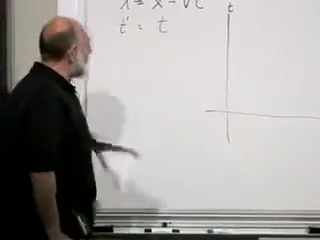
\includegraphics[width=0.72\textwidth]{lecture_04_figure_02.png}
\caption{$t$-$x$ 초기 격자와 갈릴레이 변환. 움직이는 원점은 $x=vt$을 따라가며, 두 기준계는 동일한 일정 시간선을 유지합니다.}
\lectureframe{00:03:06}
\end{figure}

식~\eqref{eq:l4-galilean}에서 프라임이 없는 좌표를 구하면 다음과 같습니다.
\begin{align}
x&=x'+vt'=x'+vt, & t&=t'.
\end{align}
역변환은 $v$을 $-v$로 바꾸면 같은 형태가 됩니다. 기차가 역에 대해 앞으로 움직이면 역은 기차에 대해 뒤로 움직입니다. 이 상호성은 특수 상대성 이론에서도 유지되지만, 보편적 시간은 그렇지 않습니다.

\section{로런츠 보정}

갈릴레이 변환으로는 모든 관성계에서 빛의 속도가 같게 되지 않습니다. 보정된 관계식은 먼저 $c=1$ 단위로 쓰면 다음과 같습니다.
\begin{align}
x'&=\frac{x-vt}{\sqrt{1-v^2}}, &
t'&=\frac{t-vx}{\sqrt{1-v^2}}.
\label{eq:l4-lorentz-natural}
\end{align}
일반적인 단위로 되돌리면 다음과 같습니다.
\begin{align}
x'&=\frac{x-vt}{\sqrt{1-v^2/c^2}}, &
t'&=\frac{t-vx/c^2}{\sqrt{1-v^2/c^2}}.
\label{eq:l4-lorentz-c}
\end{align}

\begin{figure}[H]
\centering
\includegraphics[width=0.74\textwidth]{lecture_04_figure_05.png}
\caption{인자 $c$를 다시 넣은 로런츠 변환.}
\lectureframe{00:09:10}
\end{figure}

$v\ll c$일 때, 뉴턴 역학이 적용되는 상황에서는 $v^2/c^2$과 $vx/c^2$가 모두 매우 작습니다. 그러면 식~\eqref{eq:l4-lorentz-c}은 갈릴레이 결과로 환원됩니다. 상대성 이론은 뉴턴 운동학을 폐기하지 않고, 그 유효 범위를 밝혀 줍니다.

$v=c$에서는 분모가 영이 된다. 관성계는 다른 관성계에 대해 빛의 속도로 움직일 수 없다. 그 한계에서 충분히 멀리 떨어져 있으면 보정은 작지만, 한계에 가까워지면 $x$와 $t$의 혼합을 피할 수 없다.

운동 방향을 $x$로 정했으므로, 횡방향 좌표는 변하지 않습니다.
\begin{equation}
y'=y,\qquad z'=z.
\end{equation}
그 이유를 살펴보는 한 가지 방법은 기차와 승강장에 똑같은 횡방향 미터자를 놓는 것입니다. 두 기준계의 중간에서 움직이는 관측자는 막대들이 서로 반대 방향으로 같은 속도로 다가오는 것을 봅니다. 이 설정에는 어느 한쪽 횡방향 막대를 다른 쪽보다 짧게 만들 만한 특징이 없습니다.

\section{빛원뿔을 따른 로런츠 변환}

식~\eqref{eq:l4-lorentz-natural}을 기하학적으로 읽는 방법이 있습니다. 두 식을 더하면 다음과 같습니다.
\begin{align}
t'+x'
&=\frac{(t-vx)+(x-vt)}{\sqrt{1-v^2}}\\
&=(t+x)\frac{1-v}{\sqrt{1-v^2}}\\
&=(t+x)\sqrt{\frac{1-v}{1+v}}.
\label{eq:l4-null-plus}
\end{align}
이번에는 순서를 바꾸어 빼면 다음과 같습니다.
\begin{align}
t'-x'
&=\frac{(t-vx)-(x-vt)}{\sqrt{1-v^2}}\\
&=(t-x)\frac{1+v}{\sqrt{1-v^2}}\\
&=(t-x)\sqrt{\frac{1+v}{1-v}}.
\label{eq:l4-null-minus}
\end{align}

\begin{figure}[H]
\centering
\includegraphics[width=0.75\textwidth]{lecture_04_figure_06.png}
\caption{영벡터 조합 $t+x$과 $t-x$로 다시 쓴 로런츠 변환. 두 조합의 스케일 인자는 서로 역수입니다.}
\lectureframe{00:18:45}
\end{figure}

조합 $t+x$과 $t-x$은 두 $45^\circ$ 광선 방향을 따른 좌표입니다. 부스트는 이 방향 중 하나를 수축시키고 다른 하나를 역수 인자만큼 늘립니다. 어느 방향도 $45^\circ$에서 벗어나 회전하지 않습니다. 따라서 빛선은 계속 빛선으로 남으며, 이것이 빛의 불변 속도를 보여 주는 시공간 그림입니다.

\begin{classroomqa}\audiencequestion{중간 기준계의 관측자가 대칭적인 실험을 본다고 해서, 기차와 승강장 관측자에게도 같은 결과가 성립한다는 점을 어떻게 알 수 있나요?\lecturetimestamp{00:20:48}}\lecturerresponse{여기에는 한 가지 사실이 더 쓰입니다. 사건의 일치는 불변입니다. 막대의 양 끝이 만나면, 그 만남은 하나의 시공간 사건입니다. 모든 관성 관측자는 그 사건에 서로 다른 좌표를 부여할 수 있지만, 하나의 일치를 서로 다른 두 위치로 나눌 수는 없습니다. 서로 대응하는 끝점이 만나는 곳에서 섬광을 내보내면 그 사건을 실험적으로 검출할 수 있습니다. 중간 기준계의 대칭성과 두 끝점 만남의 불변성으로 횡방향 길이가 같음을 알 수 있습니다.}\end{classroomqa}

\begin{classroomqa}\audiencequestion{중간 기준계를 나타내는 자전거 타는 사람은 실제로 막대의 중간 지점에 있어야 하나요?\lecturetimestamp{00:22:25}}\lecturerresponse{아닙니다. 기준계란 한곳에 있는 한 사람의 눈이 아니라, 관측자와 시계로 이루어진 전체 네트워크입니다. 자전거 타는 사람은 끝점에서 나온 섬광을 나중에 받아 그 섬광이 어디서 나왔는지 추론할 수 있습니다. 중요한 것은 빛을 나중에 받은 위치가 아니라 각 방출 사건의 시공간상 위치입니다.}\end{classroomqa}

연속된 속도를 합성하는 일도 같은 변환에서 나오는 결과지만, 다음 강의로 미루겠습니다. 이번에는 움직이는 시계가 측정하는 불변량을 확인하는 것이 목표입니다.

\section{불변 간격}

일반적인 데카르트 좌표축을 회전하면 양 $x^2+y^2$는 변하지 않습니다. 로런츠 변환은 다른 이차 형식을 보존합니다. 식~\eqref{eq:l4-lorentz-natural}에서
\begin{align}
t'^2-x'^2
&=\frac{(t-vx)^2-(x-vt)^2}{1-v^2}\\
&=\frac{t^2-2vtx+v^2x^2-x^2+2vtx-v^2t^2}{1-v^2}\\
&=t^2-x^2.
\label{eq:l4-interval}
\end{align}
교차항은 상쇄되고, 남은 분자에는 $1-v^2$이라는 공통 인자가 들어 있습니다.

\begin{figure}[H]
\centering
\includegraphics[width=0.76\textwidth]{lecture_04_figure_07.png}
\caption{$t'^2-x'^2=t^2-x^2$의 판서 유도.}
\lectureframe{00:33:15}
\end{figure}

공간 차원이 세 개일 때 불변량은 다음과 같습니다.
\begin{equation}
t'^2-x'^2-y'^2-z'^2=t^2-x^2-y^2-z^2
\end{equation}
$c=1$ 단위에서 그렇습니다. 더 일반적으로 두 사건 사이에는 좌표 차이를 사용합니다.
\begin{equation}
\Delta s^2
=c^2\Delta t^2-\Delta x^2-\Delta y^2-\Delta z^2.
\label{eq:l4-spacetime-interval}
\end{equation}
각 관성 관측자는 시간 항과 공간 항의 값에는 동의하지 않더라도 이 수치에는 동의합니다.

\section{고유 시간과 움직이는 시계}

빛 신호를 주고받아 시계를 동기화한 정지 관측자들의 격자를 생각해 봅시다. 이들의 시계가 가리키는 값으로 좌표 시간 $t$를 정합니다. 이제 손목시계 하나를 그 격자 안에서 움직여 봅시다. 손목시계 자체의 표시는 그 세계선을 따라가며, 그 표시가 고유 시간입니다.

시간꼴로 분리된 두 사건에 대해 다음과 같이 정의합니다.
\begin{equation}
c^2\Delta\tau^2
=c^2\Delta t^2-\Delta x^2-\Delta y^2-\Delta z^2.
\label{eq:l4-proper-time}
\end{equation}
$c=1$인 한 공간 차원에서는 단순히 다음과 같습니다.
\begin{equation}
\Delta\tau=\sqrt{\Delta t^2-\Delta x^2}.
\end{equation}
제곱근은 보통 거리의 공식과 비슷하지만, 마이너스 부호 때문에 기하학이 달라집니다.

경우는 세 가지입니다.
\begin{align}
\Delta t^2-\Delta x^2 &>0 &&\text{timelike},\\
\Delta t^2-\Delta x^2 &=0 &&\text{lightlike},\\
\Delta t^2-\Delta x^2 &<0 &&\text{spacelike}.
\end{align}
빛원뿔 안쪽에서는 고유 시간이 실수입니다. 원뿔 위에서는 $x=\pm t$이므로 사건들이 일치하지 않아도 고유 시간은 0입니다. 빛선은 바로 이런 사건들을 연결할 수 있습니다. 원뿔 바깥쪽에서는 분리가 공간꼴입니다. 이때는 시계 시간의 허수값보다 실수인 고유 거리 $\sqrt{\Delta x^2-\Delta t^2}$로 나타내는 편이 적절합니다.

\begin{figure}[H]
\centering
\includegraphics[width=0.73\textwidth]{lecture_04_figure_08.png}

\vspace{0.8em}

\begin{tikzpicture}[x=1.0cm,y=1.0cm]
\draw[->] (-3.3,0) -- (3.3,0) node[right] {$x$};
\draw[->] (0,-0.4) -- (0,4.0) node[above] {$t$};
\draw[thick] (0,0) -- (3.0,3.0) node[above right] {$x=t$};
\draw[thick] (0,0) -- (-3.0,3.0) node[above left] {$x=-t$};
\node at (0,2.0) {timelike};
\node at (2.25,1.05) {spacelike};
\node at (-2.25,1.05) {spacelike};
\end{tikzpicture}\caption{시간꼴, 빛꼴, 공간꼴 분리를 명확하게 구분한 판서 빛원뿔.}\lectureframe{00:38:40}
\end{figure}

식~\eqref{eq:l4-proper-time}은 왜 시계의 표시와 같을까요? 정지한 시계에서는 $\Delta x=0$이므로 $\Delta\tau=\Delta t$입니다. 등속 운동하는 시계의 경우, 그 시계가 정지해 있는 프라임 좌표계를 택합시다. 그 좌표계에서는 $\Delta x'=0$이고, 불변성에 따라
\begin{equation}
\Delta\tau
=\sqrt{\Delta t'^2-\Delta x'^2}
=\Delta t'.
\end{equation}
따라서 움직이는 시계가 기록하는 것은 고유 시간입니다.

\begin{classroomqa}\audiencequestion{``사건 사이의 간격''과 ``시계가 가리키는 값''은 같은 것을 가리키는 두 가지 이름인가요?\lecturetimestamp{00:44:49}}\lecturerresponse{이상적인 시계가 한 사건에서 다른 사건까지 관성 운동을 하면 두 값은 일치합니다. 불변 간격은 기하학적 양이고, 함께 움직이는 시계의 두 끝점 표시 차이는 그 양을 물리적으로 측정한 값입니다. 정지한 좌표계의 시계는 일반적으로 이와 다른 좌표 시간 간격을 기록합니다.}\end{classroomqa}

\section{시간 지연과 동시성}

움직이는 좌표계의 원점을 생각해 봅시다. 그 세계선은 다음 관계를 따릅니다.
\begin{equation}
x'=0,\qquad x=vt.
\end{equation}
기울어진 이 선은 움직이는 시계의 경로이자 $t'$축입니다.

\begin{figure}[H]
\centering
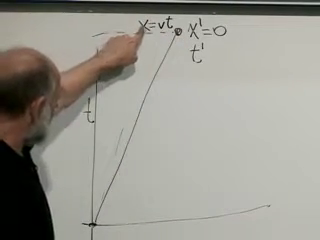
\includegraphics[width=0.72\textwidth]{lecture_04_figure_03.png}
\caption{움직이는 원점: $x=vt$, $x'=0$, $t'$축은 모두 같은 세계선을 가리키는 세 가지 표현입니다.}
\lectureframe{00:48:18}
\end{figure}

공통 원점과 그 세계선 위의 나중 점 사이에 불변 간격을 적용하면 다음과 같습니다.
\begin{align}
t'^2-x'^2&=t^2-x^2,\\
t'^2&=t^2-v^2t^2,\\
t'&=t\sqrt{1-v^2}.
\label{eq:l4-time-dilation-natural}
\end{align}
$c$를 다시 표시하면
\begin{equation}
\Delta\tau=\Delta t\sqrt{1-\frac{v^2}{c^2}}
=\frac{\Delta t}{\gamma},
\qquad
\gamma=\frac{1}{\sqrt{1-v^2/c^2}}.
\label{eq:l4-time-dilation}
\end{equation}

\begin{figure}[H]
\centering
\includegraphics[width=0.73\textwidth]{lecture_04_figure_09.png}
\caption{판서에 나온 시간 지연 결과: $c=1$ 단위에서 움직이는 시계가 누적하는 시간은 $t'=t\sqrt{1-v^2}$입니다.}
\lectureframe{00:50:45}
\end{figure}

정지 관측자는 움직이는 시계가 느리게 간다고 말합니다. 상호성에 따라 움직이는 관측자도 정지한 시계가 느리게 간다고 말해야 합니다. 두 설명은 서로 다른 원거리 사건 쌍을 비교하므로 모순이 아닙니다.

실제로 식~\eqref{eq:l4-lorentz-natural}에서 $t'$가 일정한 값이면 다음 관계를 만족합니다.
\begin{equation}
t-vx=\text{constant}.
\label{eq:l4-simultaneity}
\end{equation}
움직이는 관측자의 동시성 선은 수평선 $t=\text{constant}$에 대해 기울어져 있습니다. 관측자마다 서로 다른 원거리 시계 표시들을 동시에 일어난 것으로 봅니다. 이 차이를 분명히 해 두면 시계가 서로에게 상대적으로 느리게 간다는 결과는 모순 없이 양립합니다.

\begin{figure}[H]
\centering
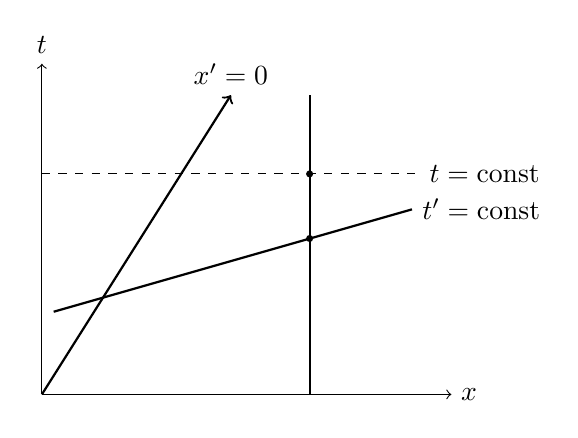
\begin{tikzpicture}[x=1cm,y=1cm]
\draw[->] (0,0) -- (0,4.2) node[above] {$t$};
\draw[->] (0,0) -- (5.2,0) node[right] {$x$};
\draw[thick,->] (0,0) -- (2.4,3.8) node[above] {$x'=0$};
\draw[dashed] (0,2.8) -- (4.8,2.8)
  node[right] {$t=\mathrm{const}$};
\draw[thick] (0.15,1.05) -- (4.7,2.35)
  node[right] {$t'=\mathrm{const}$};
\draw[thick] (3.4,0) -- (3.4,3.8);
\fill (3.4,2.8) circle (0.045);
\fill (3.4,1.98) circle (0.045);
\end{tikzpicture}
\caption{상호적 시간 지연은 서로 다른 동시성 단면 위의 시계 표시를 비교합니다.}
\end{figure}

\section{쌍둥이의 경로}

두 쌍둥이는 같은 사건에서 출발합니다. 한 명은 $x=0$에 머뭅니다. 다른 한 명은 속도 $v$로 바깥쪽으로 이동했다가 방향을 바꾸어 같은 속도로 돌아옵니다. 다시 만났을 때 손목시계, 심장 박동, 신진대사, 노화 자체처럼 시계 역할을 할 수 있는 모든 물리적 과정의 결과를 비교합니다.

집에 남은 쌍둥이의 기준계에서 여정의 각 절반이 좌표 시간 $T$만큼 걸린다고 합시다. 집에 남은 쌍둥이의 고유 시간은 다음과 같습니다.
\begin{equation}
\tau_{\mathrm{home}}=2T.
\end{equation}
방향을 바꾸는 사건의 좌표는 $(vT,T)$입니다. 따라서 여행의 첫 구간에서 누적되는 고유 시간은
\begin{align}
\tau_{\mathrm{leg}}
&=\sqrt{T^2-v^2T^2}
=T\sqrt{1-v^2}.
\end{align}
돌아오는 구간에서도 같은 만큼 누적되므로
\begin{equation}
\tau_{\mathrm{travel}}=2T\sqrt{1-v^2}<2T.
\label{eq:l4-twin}
\end{equation}

\begin{figure}[H]
\centering
\includegraphics[width=0.73\textwidth]{lecture_04_figure_10.png}

\vspace{0.8em}

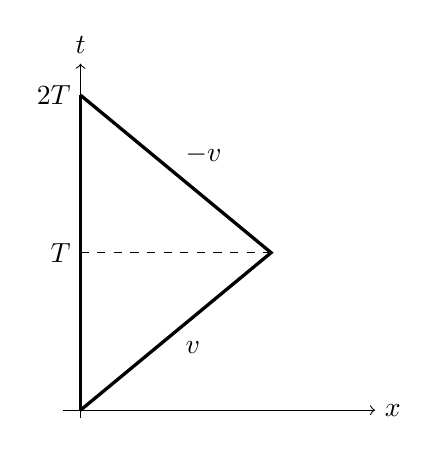
\begin{tikzpicture}[x=1.1cm,y=1cm]
\draw[->] (-0.2,0) -- (3.4,0) node[right] {$x$};
\draw[->] (0,-0.1) -- (0,4.4) node[above] {$t$};
\draw[very thick] (0,0) -- (0,4);
\draw[very thick] (0,0) -- (2.2,2) -- (0,4);
\draw[dashed] (0,2) -- (2.2,2);
\node[left] at (0,2) {$T$};
\node[left] at (0,4) {$2T$};
\node[below right] at (1.1,1.0) {$v$};
\node[above right] at (1.1,3.0) {$-v$};
\end{tikzpicture}\caption{집에 남은 쌍둥이의 세계선과 여행자의 두 구간. 시공간을 지나는 경로가 서로 다르므로 이들의 고유 시간도 다릅니다.}\lectureframe{00:59:35}
\end{figure}

나이가 서로 달라도 모순은 없습니다. 여행자의 경로에는 방향 전환이 있고, 하나의 관성계 대칭 변환으로 집에 남은 쌍둥이의 직선 경로와 연결되지 않습니다. 보통의 유클리드 기하에서도 두 점을 잇는 직선 경로와 꺾인 경로의 길이는 다릅니다. 민코프스키 기하에서는 어느 경로의 간격이 더 큰지가 반대가 되지만, 비교 자체는 여전히 기하학적입니다.

\section{가속과 이상적인 시계}

\begin{classroomqa}\audiencequestion{방향을 바꾸는 순간에는 물리가 달라지고 여행자가 가속합니다. 그러면 시계 계산이 무효가 되나요?\lecturetimestamp{01:02:19}}\lecturerresponse{가속은 실제로 존재하며 비대칭을 드러내는 데 도움이 됩니다. 가속을 없던 일처럼 취급해서는 안 됩니다. 날카로운 모서리는 이상화한 그림일 뿐이므로 유한한 시간 동안 부드럽게 방향을 바꾸도록 그릴 수 있습니다. 여기에는 추가적인 물리적 가정도 필요합니다. 충분히 작고 잘 만들어진 시계는 적당한 가속에 민감하지 않아 계속 고유 시간을 기록한다는 가정입니다. 크거나 깨지기 쉬운 시계는 변형되거나 망가질 수 있지만, 그것은 시공간 간격의 문제가 아니라 시계 장치의 결함입니다.}\end{classroomqa}

이 이상적인 시계에 관한 가정은 로런츠 변환만으로 유도되지 않습니다. 실제 시계 장치의 거동을 통해 검증해야 합니다. 원자는 수백 마일 크기의 시계보다 훨씬 좋은 근사물입니다. 작은 장치는 가속이나 중력으로 변형되기 어렵기 때문입니다. 일반 상대성 이론을 언급한다고 해서 이 물리적 문제가 사라지는 것은 아닙니다. 선택한 장치가 주변 환경에 어떻게 반응하는지 여전히 알아야 합니다.

\begin{classroomqa}\audiencequestion{가속하는 궤적을 짧은 구간들로 나누어 각 구간에서 관성계 분석을 적용할 수 있나요?\lecturetimestamp{01:09:08}}\lecturerresponse{가능합니다. 곡선을 짧고 거의 직선인 구간들로 나누어 각 구간의 고유 시간을 계산한 다음, 결과를 더하면 됩니다. 이는 많은 짧은 선분으로 보통 곡선의 길이를 구하는 것과 비슷한 시공간상의 방법입니다. 연속체 극한에서는
\[
\tau=\int \sqrt{1-\frac{v(t)^2}{c^2}}\,dt,
\]
관성 좌표계로 기술하는 평탄한 시공간에서의 운동에 대해 이 식이 성립합니다.}\end{classroomqa}

\section{쌍둥이가 보는 것}

빛 펄스를 보내면 최종 시계 표시를 실험적으로 확인할 수 있습니다. 두 세계선에서 고유 시간 1초 간격을 표시하고, 쌍둥이 각자가 표시가 있을 때마다 펄스를 내보내게 합시다. 바깥쪽으로 가는 동안에는 상대방에게서 받은 펄스 사이 간격이 벌어집니다. 돌아오는 동안에는 펄스가 뭉쳐서 도착합니다. 이는 시공간 그림에 직접 나타낸 상대론적 도플러 효과입니다.

\begin{figure}[H]
\centering
\includegraphics[width=0.73\textwidth]{lecture_04_figure_11.png}
\caption{집에 남은 쌍둥이와 여행자의 세계선 사이에서 주고받는 빛 신호. 바깥쪽으로 가는 구간에서는 펄스가 드문드문 도착하고, 돌아오는 구간에서는 도착 간격이 줄어듭니다. 이로써 방출된 모든 펄스를 빠짐없이 설명할 수 있습니다.}
\lectureframe{01:12:55}
\end{figure}

이 이야기의 어떤 시간 구간도 사라지지 않습니다. 각 관측자는 결국 상대방이 보낸 모든 펄스를 받지만, 수신율은 상대 운동에 따라 달라집니다. 두 경로에서 적색편이와 청색편이가 지속되는 시간은 같지 않으므로, 받은 펄스를 모두 세면 고유 시간 비교와 일치합니다.

\begin{classroomqa}\audiencequestion{돌아오는 여행자가 청색편이된 빛을 받는다면, 방출원이 낸 에너지보다 더 많은 에너지를 얻을 수 있나요?\lecturetimestamp{01:13:50}}\lecturerresponse{이 질문에 답하려면 아직 다루지 않은 에너지의 상대론적 정의와 기준계 의존성을 알아야 합니다. 타당한 질문이지만, 특히 가속 관측자의 경우 좌표와 펄스 수만으로는 에너지 수지를 따질 수 없습니다. 그러므로 답을 추측하기보다 뒤로 미루어야 합니다.}\end{classroomqa}

\section{닫힌 공간 방향}

\begin{classroomqa}\audiencequestion{공간 방향 하나가 콤팩트하다고 합시다. 쌍둥이 한 명이 그 방향을 따라 등속 운동하여 출발점으로 돌아오면서 가속을 완전히 피할 수 있을까요? 그렇다면 두 쌍둥이를 구별하는 것은 무엇인가요?\lecturetimestamp{01:15:14}}\lecturerresponse{공간은 더 큰 공간 안에 구부러진 면이 아니라, 그 자체로 원통인 공간으로 상상해야 합니다. 방사 방향 가속은 없어도 됩니다. 그래도 돌아온 관측자는 같은 장소가 되풀이된다는 전역적 사실을 마주하게 됩니다. 이는 비대칭이 있음을 보여 주지만, 완전한 답을 위해서는 공간을 동일시하는 특수 상대성 이론을 신중하게 다루어야 합니다. 여기서는 즉흥적으로 답하지 않고 열린 질문으로 남겨 둡니다.}\end{classroomqa}

\begin{figure}[H]
\centering
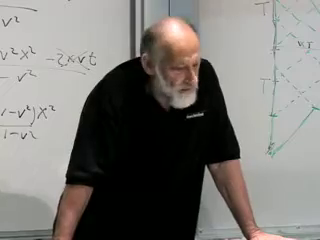
\includegraphics[width=0.72\textwidth]{lecture_04_figure_04.png}

\vspace{0.8em}

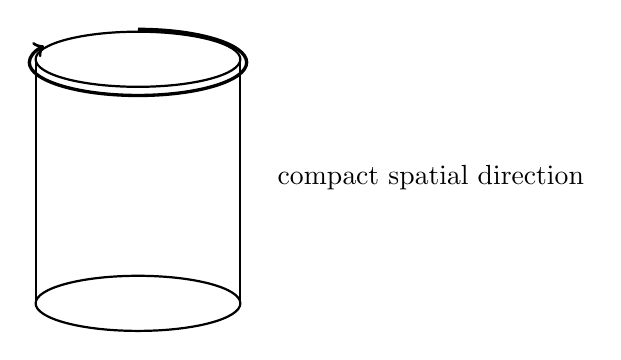
\begin{tikzpicture}[x=1cm,y=1cm]
\draw[thick] (0,0) ellipse (1.3 and 0.35);
\draw[thick] (-1.3,0) -- (-1.3,-3.1);
\draw[thick] (1.3,0) -- (1.3,-3.1);
\draw[thick] (0,-3.1) ellipse (1.3 and 0.35);
\draw[->,very thick] (0.0,0.38) arc (90:-210:1.38 and 0.42);
\node[right] at (1.65,-1.5) {compact spatial direction};
\end{tikzpicture}\caption{판서에 그린 콤팩트 공간 질문과 깔끔한 내재적 원통. 이 질문은 추가적인 방사 차원에 놓인 원통 주위의 운동이 아니라 전역적 동일시에 관한 것입니다.}\lectureframe{01:17:56}
\end{figure}

\section{동시성 단면에서 측정하는 길이}

특수 상대성 이론 문제에서는 먼저 시공간 그림을 그립니다. 프라임이 없는 기준계에서 정지해 있는 미터자를 생각해 봅시다. 양 끝점은 $x=0$과 $x=1$에 있습니다. 시간이 흐르면 두 끝점은 수직 세계선을 그립니다. 막대는 그 사이의 시공간 영역을 쓸어 냅니다.

움직이는 관측자는 움직이는 시간 $t'$가 한 값일 때 두 끝점을 모두 측정해야 합니다. 식~\eqref{eq:l4-simultaneity}에서 원점을 지나며 $t'=0$인 단면은 다음 관계를 만족합니다.
\begin{equation}
t=vx
\end{equation}
$c=1$ 단위에서 그렇습니다. 이 단면은 $x=1$인 오른쪽 끝점과 $t=v$에서 만납니다.

\begin{figure}[H]
\centering
\includegraphics[width=0.73\textwidth]{lecture_04_figure_12.png}

\vspace{0.8em}

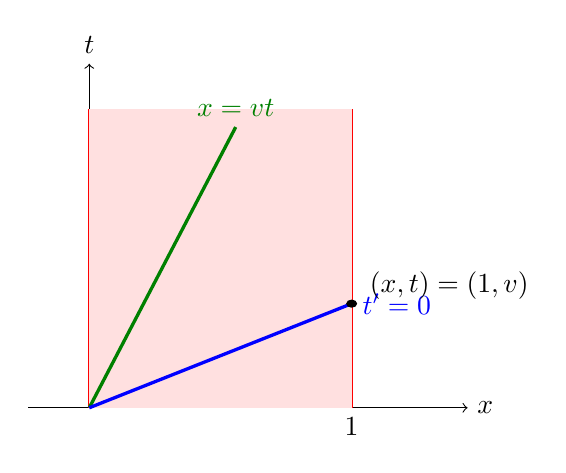
\begin{tikzpicture}[x=1.55cm,y=1.15cm]
\draw[->] (-0.5,0) -- (3.1,0) node[right] {$x$};
\draw[->] (0,0) -- (0,3.8) node[above] {$t$};
\draw[very thick,red] (0,0) -- (0,3.3);
\draw[very thick,red] (2.15,0) -- (2.15,3.3);
\fill[red!12] (0,0) rectangle (2.15,3.3);
\draw[very thick,green!50!black] (0,0) -- (1.2,3.1)
  node[above] {$x=vt$};
\draw[very thick,blue] (0,0) -- (2.15,1.15)
  node[right] {$t'=0$};
\fill (2.15,1.15) circle (0.045);
\node[right] at (2.22,1.35) {$(x,t)=(1,v)$};
\node[below] at (2.15,0) {$1$};
\end{tikzpicture}\caption{정지한 막대는 시공간 영역을 쓸어 냅니다. 움직이는 관측자가 측정하는 길이는 하나의 $t'=\mathrm{const}$ 단면에서 잰 양 끝점 사이의 간격입니다.}\lectureframe{01:24:20}
\end{figure}

선택한 두 끝점 사이의 간격은 공간꼴이므로 불변량의 양의 공간꼴 형태를 사용합니다.
\begin{equation}
x'^2-t'^2=x^2-t^2.
\end{equation}
선택한 끝점에서 $t'=0$, $x=1$, $t=v$입니다. 따라서
\begin{align}
x'^2&=1-v^2,\\
x'&=\sqrt{1-v^2}.
\end{align}
정지 길이 $L$는 움직이는 기준계에서 다음과 같이 측정됩니다.
\begin{equation}
L'=L\sqrt{1-v^2/c^2}=\frac{L}{\gamma}.
\label{eq:l4-length-contraction}
\end{equation}

\begin{figure}[H]\centering
\includegraphics[width=0.76\textwidth]{lecture_04_figure_13.png}\caption{완성된 길이 수축 도식과 정지 길이가 단위일 때의 판서 결과 $x'=\sqrt{1-v^2}$}\lectureframe{01:28:10}\end{figure}

상호적인 설명도 성립합니다. 승강장 관측자는 기차의 길이 방향 미터자를 더 짧게 측정합니다. 여기서도 두 관측자는 서로 다른 동시적 끝점 사건을 선택하므로 상호성이 모순을 일으키지 않습니다.

\section{마무리 질문}

\begin{classroomqa}
\audiencequestion{빛 외에 빛의 속도로 전파되는 것도 있나요? 특히 중력은 어떤가요?\lecturetimestamp{01:29:29}}
\lecturerresponse{일반 상대성 이론은 $c$의 속도로 전파되는 중력파를 예측합니다. 이 강의가 진행된 당시에는 쌍성 펄서와 같은 계에서 얻은 간접 증거가 있었지만, 중력파를 직접 검출하지는 못했습니다.\editorialnote{실험 상황은 이 2006년 강의 이후 달라졌습니다. LIGO는 GW150914를 2015년에 직접 검출했고, GW170817와 그 전자기 대응체를 함께 관측한 2017년의 관측으로 중력과 빛의 전파 속도가 $10^{15}$분의 몇 정도 이내의 차이로 일치함을 보였습니다. \url{https://ligo.org/detections/gw150914/} 및 \url{https://doi.org/10.1103/PhysRevLett.119.251302}을 참조하세요.}}\end{classroomqa}

\begin{classroomqa}\audiencequestion{우주비행사가 여러 광년 거리를 거리의 광년 수보다 짧은 고유 시간에 건널 수 있나요? 그렇다면 빛보다 빠르게 이동한 셈인가요?\lecturetimestamp{01:30:38}}\lecturerresponse{우주비행사의 고유 시간은 $\sqrt{\Delta t^2-\Delta x^2}$이며, 이는 좌표 시간 $\Delta t$보다 짧습니다. 우주비행사의 관성계에서는 별들 사이의 거리가 로런츠 수축됩니다. 별들은 빛보다 빠른 속도가 아니라 $-v$의 속도로 움직입니다. 건너야 할 거리가 수축되어 더 짧을 뿐입니다.}\end{classroomqa}

우주비행사가 정지 상태에서 출발해 가속하면, 설명은 연속된 순간 관성계 사이에서 바뀝니다. 그 전환 동안 별들 사이의 거리도 달라질 수 있습니다. 가속하는 전체 이력에 하나의 고정된 로런츠 변환을 적용할 수는 없지만, 세계선을 따라 누적되는 고유 시간은 각 구간의 기여분을 더해 구할 수 있습니다. 이 설명은 순항 속도로 태어나는 대신 발사하고 방향을 바꾸어 감속하는 현실적인 쌍둥이에게도 적용됩니다.

\begin{classroomqa}\audiencequestion{시간을 특별하게 취급하기 때문에 이런 역설이 생기나요? 시간을 4차원이라고 불러야 하나요?\lecturetimestamp{01:36:43}}\lecturerresponse{시간을 4차원이라고 부르는 구호에서 시작할 필요는 없습니다. 로런츠 변환 자체가 공간과 시간을 서로 섞이게 하며, 간격 $t^2-x^2-y^2-z^2$은 시간과 공간에 서로 다른 부호를 부여해 이들을 하나의 기하학 안에 놓습니다. 속도가 낮으면 혼합 효과가 무시할 만큼 작아져 익숙한 뉴턴적 직관이 되살아납니다. 그러나 상대론적 속도에서는 공간과 시간을 근본적으로 분리된 것으로 볼 수 없습니다.}\end{classroomqa}

따라서 시간 지연, 길이 수축, 쌍둥이 비교, 짧아진 여행 시간은 서로 별개의 요령이 아닙니다. 비교할 사건을 식별하고, 시공간 기하를 그리며, 불변 간격을 사용한다는 세 가지 원칙에서 모두 따라 나옵니다.